\documentclass[a4paper]{article}

%% Language and font encodings
\usepackage[french]{babel}
\usepackage[utf8x]{inputenc}
\usepackage[T1]{fontenc}
\usepackage{wrapfig}

%% Sets page size and margins
\usepackage[a4paper,top=3cm,bottom=2cm,left=3cm,right=3cm,marginparwidth=1.75cm]{geometry}

%% Useful packages
\usepackage{amsmath}
\usepackage{graphicx}
\usepackage[colorinlistoftodos]{todonotes}
\usepackage[colorlinks=true, allcolors=blue, breaklinks=true]{hyperref}

\newcommand{\guill}[1]{\og{}#1\fg{}}

\title{Le planning de ma cuisine}
\author{Adrien Krähenbühl \and Basile Sauvage \and Julien Narboux}

\begin{document}
\maketitle

\begin{abstract}
Description d'une activité d'informatique débranchée sur le thème de l'ordonnancement.
\end{abstract}


\section{Notions abordées}

Algorithme, Ordonnancement, Complexité, 

\section{Description du jeu}

On se trouve dans une cuisine avec un ensemble de plats à préparer qui nécessitent chacun un certain temps de préparation et un certain temps de cuisson. Un seul plat peut être préparé à la fois, de même que le four ne peut accueillir qu'un plat à la fois.

L'objectif est de trouver l'ordre de préparation des plats qui permet de terminer l'ensemble des plats le plus rapidement possible.

\section{Matériel}

La matériel consiste en la matérialisation d'un diagramme permettant de réprésenter la plannification des tâches (ce genre de diagramme est appelé diagramme de Gantt).

Les temps de cuisson et de préparation des plats sont matérialisés par des rectangles de longueur proportionelle à la durée. Les temps de préparation sont indiqués par une toque, les temps de cuisson par un four.

Le matériel peut être construit en bois pour une utilisation intensive ou simplement en papier pour une activité en classe, des patrons sont fournis en annexe.

Le montage que nous avons réalisé consiste en une baguette de 67mm de large, trois baguettes de 9mmx9mm qui servent de guide et des rectangles découpés dans des baquettes de 18mm de large ce qu'il laisse 67-3*9-2*18=4mm de marge pour que les baguettes coulissent facilement. A refaire, il vaudrait mieux avoir une largeur différente pour les temps de préparation et les temps de cuisson, comme çà les participants ne peuvent pas se tromper.

Le meilleur temps possible pour chaque défi est indiqué par une marque sur une règle donnant l'échelle de temps.


\section{Déroulement de l'activité}

Nous proposons quatre défis et quelques questions et explications:
\begin{enumerate}
\item On explique les règles du jeu en choisissant un ordre pas optimal sur un exemple.
\item Un premier défi (croissant, brioche, pain). Si on trie les plats par ordre de temps de préparation croissant, on obtient une solution optimale.
\item Un deuxième défi (tarte flambée, jambonneau, bretzel) montre que trier par temps de préparation croissant n'est pas toujours optimal, mais si on trie par temps de cuisson décroissant cela fonctionne sur cet exemple.
\item Un troisième défi (poulet, gâteau, poisson) dont la solution optimale n'est ni un tri croissant des temps de préparation, ni un tri décroissant des temps de cuisson.
{\huge Il faut qu'on change les chiffres c'est pas le cas actuellement !}
\item Un quatrième défi (avec les 9 plats) permet de faire chercher un peu plus les participants.
\item On peut alors demander combien il y a d'ordonnancement des six plats possibles.
\item On explique l'algorithme de Johnson et on commence à l'éxecuter sur l'exemple.
\item On peut éventuellement poser la question de la complexité de l'algorithme.
\item A la fin on peut ouvrir en expliquant ce qu'est un algorithme, citer quelques applications et parler de problèmes NP-Complets 
\end{enumerate}

\section{Contexte scientifique}

TODO

\section{Retour d'expériences}

Cette activité a été testée avec le public d'un Village des Science. Le public a été assez attiré par l'installation. Les gens n'ont pas eu de mal à comprendre les règles. Les enfants à partir de 7-8 arrivent à résoudre les défis.

\begin{figure}
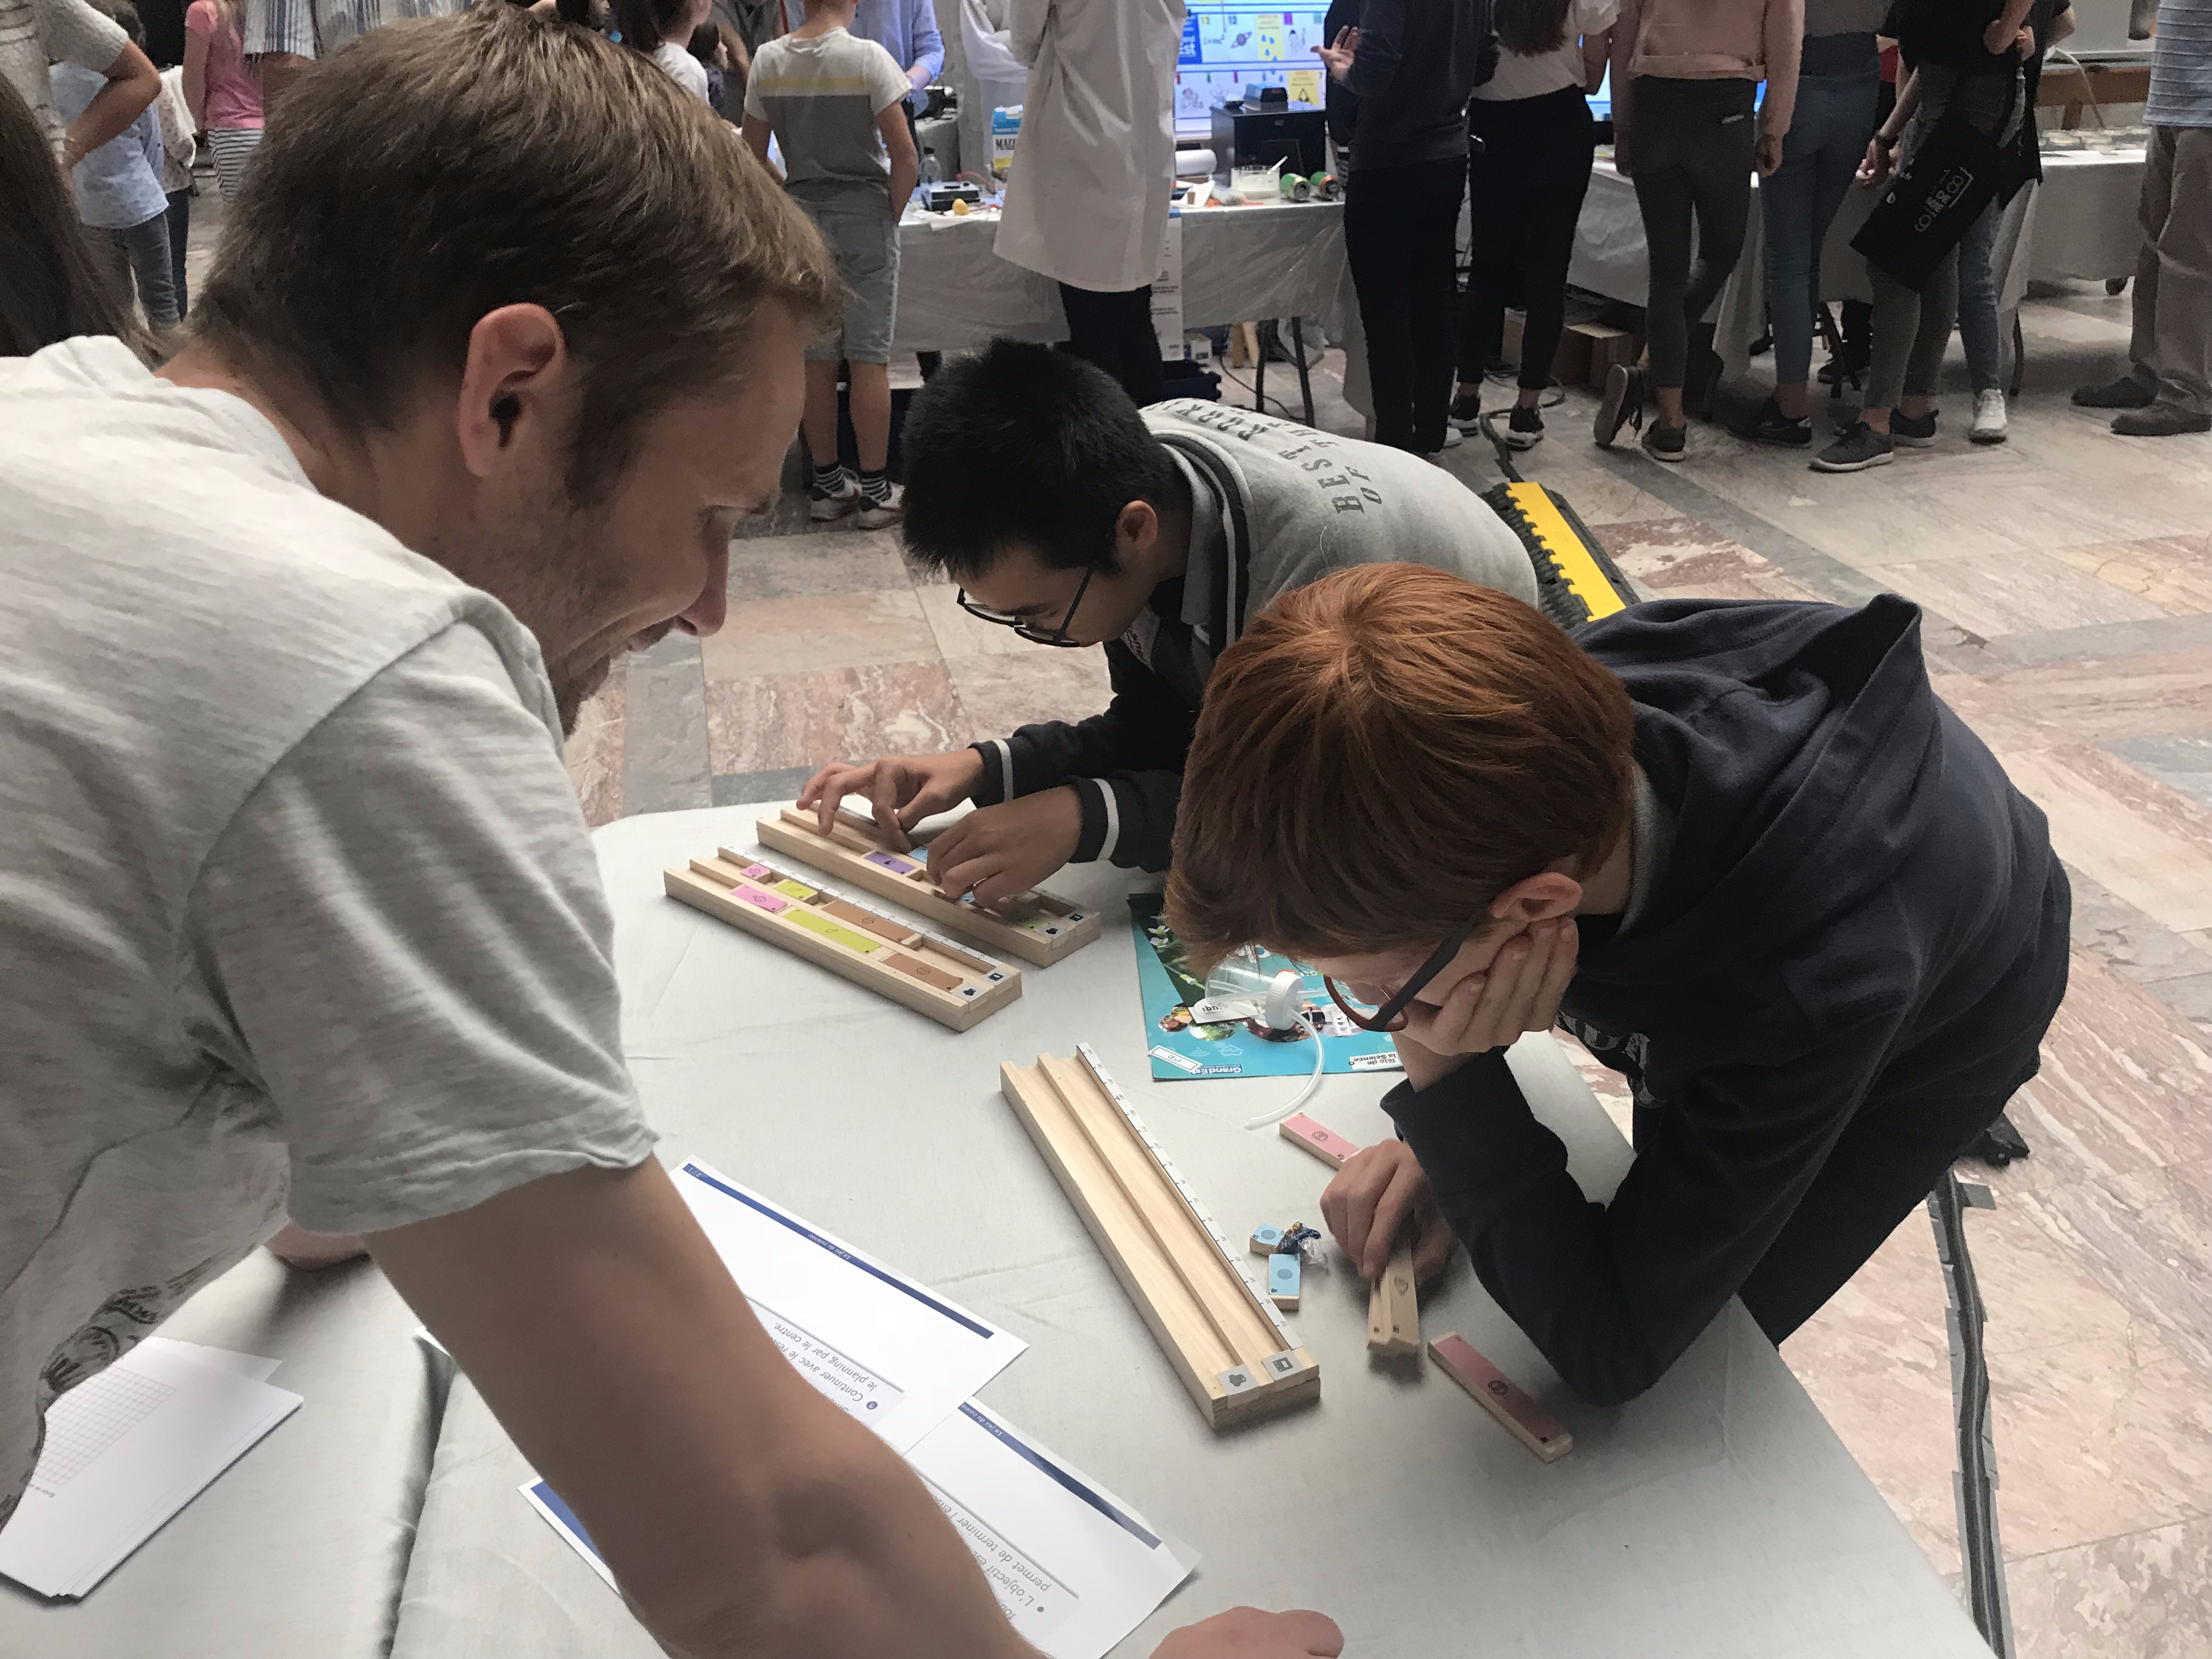
\includegraphics[width=0.5\textwidth]{IMG_2989.png}
\caption{Fête de la Science 2018, Strasbourg}
\end{figure}

\section{Pistes d'extensions}

On pourrait envisager d'ajouter à cette activité une deuxième étape avec des graphes de dépendances entre tâches.

\section{Bibliographie}

\end{document}